
\begin{table*}[h]
    
~~~~~~~~~~~~~~~~~~~~~~~~~~~~
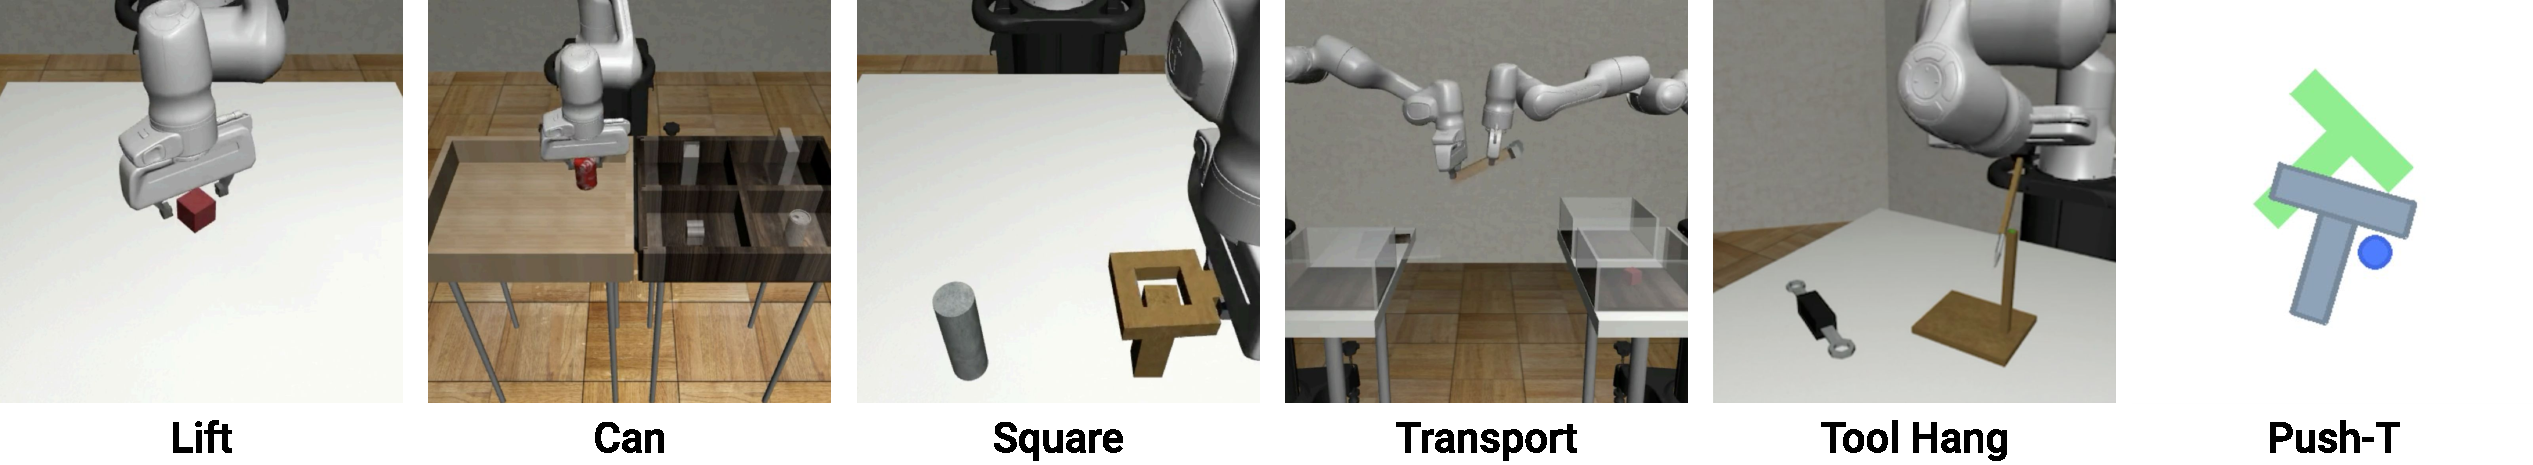
\includegraphics[width=0.82\linewidth]{figure/sim_task_thumbnails.pdf}
\label{tab:sim_benchmark_state}

\vspace{1mm}
{
\centering
% \setlength\tabcolsep{ 4.4 pt}
% \begin{tabular}{r|cc|cc|cc|cc|c|c}
% \toprule

%  & \multicolumn{2}{c|}{ Lift} & \multicolumn{2}{c|}{ Can} & \multicolumn{2}{c|}{ Square} & \multicolumn{2}{c|}{ Transport} & \multicolumn{1}{c|}{ ToolHang} & \multicolumn{1}{c}{ PushT} \\
%  & ph & mh & ph & mh & ph & mh & ph & mh & ph & ph \\
% \midrule
% LSTM-GMM \cite{robomimic} & \small \textbf{1.00}/.960 & \small \textbf{1.00}/.926 & \small \textbf{1.00}/.912 & \small \textbf{1.00}/.806 & \small .955/.732 & \small .864/.588 & \small .758/.467 & \small .621/.199 & \small .667/.312 & \small .896/.832 \\
% IBC  \cite{ibc} & \small .000/.000 & \small .000/.000 & \small .000/.000 & \small .000/.000 & \small .000/.000 & \small .000/.000 & \small .000/.000 & \small .000/.000 & \small .000/.000 & \small .000/.000 \\
% BET & \small \textbf{1.00}/.961 & \small \textbf{1.00}/.992 & \small \textbf{1.00}/.892 & \small \textbf{1.00}/.897 & \small .758/.520 & \small .682/.427 & \small .379/.145 & \small .212/.064 & \small .576/.200 & \small .797/.713 \\
% \midrule
% DiffusionPolicy-C & \small \textbf{1.00}/.985 & \small \textbf{1.00}/.970 & \small \textbf{1.00}/.959 & \small \textbf{1.00}/\textbf{.961} & \small \textbf{1.00}/\textbf{.929} & \small \textbf{.970}/\textbf{.821} & \small .939/.821 & \small \textbf{.682}/\textbf{.455} & \small .515/.221 & \small .994/\textbf{.992} \\
% DiffusionPolicy-T & \small \textbf{1.00}/\textbf{1.00} & \small \textbf{1.00}/\textbf{.999} & \small \textbf{1.00}/\textbf{.996} & \small \textbf{1.00}/.939 & \small \textbf{1.00}/.886 & \small .955/.812 & \small \textbf{1.00}/\textbf{.841} & \small .622/.351 & \small \textbf{1.00}/\textbf{.873} & \small \textbf{1.00}/.991 \\
% \bottomrule
% \end{tabular}

% this version uses number from the original paper (Robomimic)
% \setlength\tabcolsep{ 4.4 pt}
% \begin{tabular}{r|cc|cc|cc|cc|c|c}
% \toprule
%  & \multicolumn{2}{c|}{Lift} & \multicolumn{2}{c|}{Can} & \multicolumn{2}{c|}{Square} & \multicolumn{2}{c|}{Transport} & \multicolumn{1}{c|}{ToolHang} & \multicolumn{1}{c}{PushT} \\
%  & ph & mh & ph & mh & ph & mh & ph & mh & ph & ph \\
% \midrule
% LSTM-GMM \cite{robomimic} & \small \textbf{1.00}/0.96 & \small \textbf{1.00}/0.93 & \small \textbf{1.00}/0.91 & \small \textbf{1.00}/0.81 & \small 0.84/0.73 & \small 0.78/0.59 & \small 0.71/0.47 & \small 0.65/0.20 & \small 0.19/0.31 & \small 0.67/0.61 \\
% IBC \cite{ibc} & \small 0.79/0.41 & \small 0.15/0.02 & \small 0.00/0.00 & \small 0.01/0.01 & \small 0.00/0.00 & \small 0.00/0.00 & \small 0.00/0.00 & \small 0.00/0.00 & \small 0.00/0.00 & \small 0.90/0.84 \\
% BET \cite{bet} & \small \textbf{1.00}/0.96 & \small \textbf{1.00}/0.99 & \small \textbf{1.00}/0.89 & \small \textbf{1.00}/0.90 & \small 0.76/0.52 & \small 0.68/0.43 & \small 0.38/0.14 & \small 0.21/0.06 & \small 0.58/0.20 & \small 0.79/0.70 \\
% \midrule
% DiffusionPolicy-C & \small \textbf{1.00}/0.98 & \small \textbf{1.00}/0.97 & \small \textbf{1.00}/0.96 & \small \textbf{1.00}/\textbf{0.96} & \small \textbf{1.00}/\textbf{0.93} & \small \textbf{0.97}/\textbf{0.82} & \small 0.94/0.82 & \small \textbf{0.68}/\textbf{0.46} & \small 0.50/0.30 & \small 0.95/\textbf{0.91} \\
% DiffusionPolicy-T & \small \textbf{1.00}/\textbf{1.00} & \small \textbf{1.00}/\textbf{1.00} & \small \textbf{1.00}/\textbf{1.00} & \small \textbf{1.00}/0.94 & \small \textbf{1.00}/0.89 & \small 0.95/0.81 & \small \textbf{1.00}/\textbf{0.84} & \small 0.62/0.35 & \small \textbf{1.00}/\textbf{0.87} & \small \textbf{0.95}/0.79 \\
% \bottomrule
% \end{tabular}


% this version uses number we ran
\setlength\tabcolsep{ 3 pt}
\begin{tabular}{r|cc|cc|cc|cc|c|c}
\toprule
 & \multicolumn{2}{c|}{Lift} & \multicolumn{2}{c|}{Can} & \multicolumn{2}{c|}{Square} & \multicolumn{2}{c|}{Transport} & \multicolumn{1}{c|}{ToolHang} & \multicolumn{1}{c}{Push-T} \\
 & ph & mh & ph & mh & ph & mh & ph & mh & ph & ph \\
\midrule
LSTM-GMM & \small \textbf{1.00}/0.96 & \small \textbf{1.00}/0.93 & \small \textbf{1.00}/0.91 & \small \textbf{1.00}/0.81 & \small 0.95/0.73 & \small 0.86/0.59 & \small 0.76/0.47 & \small 0.62/0.20 & \small 0.67/0.31 & \small 0.67/0.61 \\
IBC & \small 0.79/0.41 & \small 0.15/0.02 & \small 0.00/0.00 & \small 0.01/0.01 & \small 0.00/0.00 & \small 0.00/0.00 & \small 0.00/0.00 & \small 0.00/0.00 & \small 0.00/0.00 & \small 0.90/0.84 \\
BET & \small \textbf{1.00}/0.96 & \small \textbf{1.00}/0.99 & \small \textbf{1.00}/0.89 & \small \textbf{1.00}/0.90 & \small 0.76/0.52 & \small 0.68/0.43 & \small 0.38/0.14 & \small 0.21/0.06 & \small 0.58/0.20 & \small 0.79/0.70 \\
\midrule
DiffusionPolicy-C & \small \textbf{1.00}/0.98 & \small \textbf{1.00}/0.97 & \small \textbf{1.00}/0.96 & \small \textbf{1.00}/\textbf{0.96} & \small \textbf{1.00}/\textbf{0.93} & \small \textbf{0.97}/\textbf{0.82} & \small 0.94/0.82 & \small \textbf{0.68}/\textbf{0.46} & \small 0.50/0.30 & \small 0.95/\textbf{0.91} \\
DiffusionPolicy-T & \small \textbf{1.00}/\textbf{1.00} & \small \textbf{1.00}/\textbf{1.00} & \small \textbf{1.00}/\textbf{1.00} & \small \textbf{1.00}/0.94 & \small \textbf{1.00}/0.89 & \small 0.95/0.81 & \small \textbf{1.00}/\textbf{0.84} & \small 0.62/0.35 & \small \textbf{1.00}/\textbf{0.87} & \small \textbf{0.95}/0.79 \\
\bottomrule
\end{tabular}

% Feb 28 update, reran diffusion cnn with obs global cond
% \setlength\tabcolsep{ 4.4 pt}
% \begin{tabular}{r|cc|cc|cc|cc|c|c}
% \toprule
%  & \multicolumn{2}{c|}{Lift} & \multicolumn{2}{c|}{Can} & \multicolumn{2}{c|}{Square} & \multicolumn{2}{c|}{Transport} & \multicolumn{1}{c|}{ToolHang} & \multicolumn{1}{c}{PushT} \\
%  & ph & mh & ph & mh & ph & mh & ph & mh & ph & ph \\
% \midrule
% LSTM-GMM \cite{robomimic} & \small \textbf{1.00}/0.96 & \small \textbf{1.00}/0.93 & \small \textbf{1.00}/0.91 & \small \textbf{1.00}/0.81 & \small 0.84/0.73 & \small 0.78/0.59 & \small 0.71/0.47 & \small 0.65/0.20 & \small 0.19/0.31 & \small 0.67/0.61 \\
% IBC \cite{ibc} & \small 0.79/0.41 & \small 0.15/0.02 & \small 0.00/0.00 & \small 0.01/0.01 & \small 0.00/0.00 & \small 0.00/0.00 & \small 0.00/0.00 & \small 0.00/0.00 & \small 0.00/0.00 & \small 0.90/0.84 \\
% BET & \small \textbf{1.00}/0.96 & \small \textbf{1.00}/0.99 & \small \textbf{1.00}/0.89 & \small \textbf{1.00}/0.90 & \small 0.76/0.52 & \small 0.68/0.43 & \small 0.38/0.14 & \small 0.21/0.06 & \small 0.58/0.20 & \small 0.79/0.70 \\
% DiffusionPolicy-C & \small \textbf{1.00}/\textbf{1.00} & \small \textbf{1.00}/0.98 & \small \textbf{1.00}/\textbf{1.00} & \small \textbf{1.00}/\textbf{0.99} & \small \textbf{1.00}/\textbf{0.95} & \small \textbf{0.98}/\textbf{0.86} & \small 0.95/\textbf{0.85} & \small \textbf{0.77}/\textbf{0.60} & \small 0.86/0.52 & \small 0.95/\textbf{0.91} \\
% DiffusionPolicy-T & \small \textbf{1.00}/\textbf{1.00} & \small \textbf{1.00}/\textbf{1.00} & \small \textbf{1.00}/1.00 & \small \textbf{1.00}/0.94 & \small \textbf{1.00}/0.89 & \small 0.95/0.81 & \small \textbf{1.00}/0.84 & \small 0.62/0.35 & \small \textbf{1.00}/\textbf{0.87} & \small \textbf{0.95}/0.79 \\
% \bottomrule
% \end{tabular}


\caption{\textbf{Behavior Cloning Benchmark (State Policy) \label{tab:table_low_dim} } 
We present success rates with different checkpoint selection methods in the format of (max performance) / (average of last 10 checkpoints), with each averaged across 3 training seeds and 50 different environment initial conditions (150 in total). 
LSTM-GMM corresponds to BC-RNN in RoboMimic\cite{robomimic}, which we reproduced and obtained slightly {better} results than the original paper. Our results show that Diffusion Policy significantly improves state-of-the-art performance across the board.
% \label{tab:table_low_dim}
% Numbers are success rate shown with different checkpoint selection methods: (max performance) / (average of last 10 checkpoints), which are then averaged across 3 training seeds and 50 different env initial conditions each (150 in total). Higher the better. LSTM-GMM correspond to BC-RNN in RoboMimic \cite{robomimic}. LSTM-GMM numbers are from our reproduction (generally slightly higher than the original paper).  \label{tab:table_low_dim}
}
\vspace{2mm}


% \setlength\tabcolsep{ 4.4 pt}
% \begin{tabular}{r|cc|cc|cc|cc|c|c}
% \toprule
%  & \multicolumn{2}{c|}{ Lift} & \multicolumn{2}{c|}{ Can} & \multicolumn{2}{c|}{ Square} & \multicolumn{2}{c|}{ Transport} & \multicolumn{1}{c|}{ ToolHang} & \multicolumn{1}{c}{ PushT} \\
%  & ph & mh & ph & mh & ph & mh & ph & mh & ph & ph \\
% \midrule
% LSTM-GMM \cite{robomimic} & \small \textbf{1.00}/.000 & \small \textbf{1.00}/.000 & \small .980/.000 & \small .960/.000 & \small .820/.000 & \small .767/.000 & \small .720/.000 & \small .420/.000 & \small .673/.000 & \small .782/.690 \\
% IBC \cite{ibc} & \small .000/.000 & \small .000/.000 & \small .000/.000 & \small .000/.000 & \small .000/.000 & \small .000/.000 & \small .000/.000 & \small .000/.000 & \small .000/.000 & \small .000/.000 \\

% \midrule
% DiffusionPolicy-C & \small \textbf{1.00}/\textbf{1.00} & \small \textbf{1.00}/\textbf{.997} & \small \textbf{1.00}/.974 & \small \textbf{1.00}/\textbf{.962} & \small .985/\textbf{.923} & \small .924/.674 & \small \textbf{.955}/.712 & \small \textbf{.697}/\textbf{.489} & \small \textbf{.849}/\textbf{.614} & \small \textbf{.984}/\textbf{.937} \\
% DiffusionPolicy-T & \small \textbf{1.00}/\textbf{1.00} & \small \textbf{1.00}/.992 & \small \textbf{1.00}/\textbf{.979} & \small \textbf{1.00}/.958 & \small \textbf{1.00}/.900 & \small \textbf{.939}/\textbf{.841} & \small .839/\textbf{.762} & \small .530/.346 & \small .712/.472 & \small .909/.810 \\
% \bottomrule
% \end{tabular}

% this version uses number from the paper
% \setlength\tabcolsep{ 4.4 pt}
% \begin{tabular}{r|cc|cc|cc|cc|c|c}
% \toprule
%  & \multicolumn{2}{c|}{Lift} & \multicolumn{2}{c|}{Can} & \multicolumn{2}{c|}{Square} & \multicolumn{2}{c|}{Transport} & \multicolumn{1}{c|}{ToolHang} & \multicolumn{1}{c}{PushT} \\
%  & ph & mh & ph & mh & ph & mh & ph & mh & ph & ph \\
% \midrule
% LSTM-GMM \cite{robomimic} & \small \textbf{1.00}/0.96 & \small \textbf{1.00}/0.95 & \small 0.98/0.88 & \small 0.96/0.90 & \small 0.82/0.59 & \small 0.77/0.38 & \small 0.72/0.62 & \small 0.42/0.23 & \small 0.67/0.49 & \small 0.69/0.54 \\
% IBC \cite{ibc} & \small 0.94/0.73 & \small 0.39/0.05 & \small 0.08/0.01 & \small 0.00/0.00 & \small 0.03/0.00 & \small 0.00/0.00 & \small 0.00/0.00 & \small 0.00/0.00 & \small 0.00/0.00 & \small 0.75/0.64 \\
% \midrule
% DiffusionPolicy-C & \small \textbf{1.00}/\textbf{1.00} & \small \textbf{1.00}/\textbf{1.00} & \small \textbf{1.00}/0.97 & \small \textbf{1.00}/0.96 & \small 0.98/\textbf{0.92} & \small \textbf{0.98}/\textbf{0.84} & \small \textbf{1.00}/\textbf{0.93} & \small \textbf{0.86}/\textbf{0.71} & \small \textbf{0.95}/\textbf{0.79} & \small \textbf{0.91}/\textbf{0.84} \\
% DiffusionPolicy-T & \small \textbf{1.00}/\textbf{1.00} & \small \textbf{1.00}/0.99 & \small \textbf{1.00}/\textbf{0.98} & \small \textbf{1.00}/\textbf{0.98} & \small \textbf{1.00}/0.90 & \small 0.94/0.80 & \small 0.98/0.81 & \small 0.71/0.48 & \small 0.76/0.47 & \small 0.78/0.66 \\
% \bottomrule
% \end{tabular}

% this version uses number from our experiments
% \setlength\tabcolsep{ 4.4 pt}
% \begin{tabular}{r|cc|cc|cc|cc|c|c}
% \toprule
%  & \multicolumn{2}{c|}{Lift} & \multicolumn{2}{c|}{Can} & \multicolumn{2}{c|}{Square} & \multicolumn{2}{c|}{Transport} & \multicolumn{1}{c|}{ToolHang} & \multicolumn{1}{c}{PushT} \\
%  & ph & mh & ph & mh & ph & mh & ph & mh & ph & ph \\
% \midrule
% LSTM-GMM \cite{robomimic} & \small \textbf{1.00}/0.96 & \small \textbf{1.00}/0.95 & \small 0.98/0.88 & \small 0.96/0.90 & \small 0.82/0.59 & \small 0.77/0.38 & \small 0.72/0.62 & \small 0.42/0.24 & \small 0.67/0.49 & \small 0.69/0.54 \\
% IBC \cite{ibc} & \small 0.94/0.73 & \small 0.39/0.05 & \small 0.08/0.01 & \small 0.00/0.00 & \small 0.03/0.00 & \small 0.00/0.00 & \small 0.00/0.00 & \small 0.00/0.00 & \small 0.00/0.00 & \small 0.75/0.64 \\
% DiffusionPolicy-C & \small \textbf{1.00}/\textbf{1.00} & \small \textbf{1.00}/\textbf{1.00} & \small \textbf{1.00}/0.97 & \small \textbf{1.00}/0.96 & \small 0.98/\textbf{0.92} & \small \textbf{0.98}/\textbf{0.84} & \small \textbf{1.00}/\textbf{0.93} & \small \textbf{0.89}/\textbf{0.69} & \small \textbf{0.95}/\textbf{0.73} & \small \textbf{0.91}/\textbf{0.84} \\
% DiffusionPolicy-T & \small \textbf{1.00}/\textbf{1.00} & \small \textbf{1.00}/0.99 & \small \textbf{1.00}/\textbf{0.98} & \small \textbf{1.00}/\textbf{0.98} & \small \textbf{1.00}/0.90 & \small 0.94/0.80 & \small 0.98/0.81 & \small 0.73/0.50 & \small 0.76/0.47 & \small 0.78/0.66 \\
% \bottomrule
% \end{tabular}

\setlength\tabcolsep{ 3 pt}
\begin{tabular}{r|cc|cc|cc|cc|c|c}
\toprule
 & \multicolumn{2}{c|}{Lift} & \multicolumn{2}{c|}{Can} & \multicolumn{2}{c|}{Square} & \multicolumn{2}{c|}{Transport} & \multicolumn{1}{c|}{ToolHang} & \multicolumn{1}{c}{Push-T} \\
 & ph & mh & ph & mh & ph & mh & ph & mh & ph & ph \\
\midrule
LSTM-GMM & \small \textbf{1.00}/0.96 & \small \textbf{1.00}/0.95 & \small \textbf{1.00}/0.88 & \small 0.98/0.90 & \small 0.82/0.59 & \small 0.64/0.38 & \small 0.88/0.62 & \small 0.44/0.24 & \small 0.68/0.49 & \small 0.69/0.54 \\
IBC & \small 0.94/0.73 & \small 0.39/0.05 & \small 0.08/0.01 & \small 0.00/0.00 & \small 0.03/0.00 & \small 0.00/0.00 & \small 0.00/0.00 & \small 0.00/0.00 & \small 0.00/0.00 & \small 0.75/0.64 \\
DiffusionPolicy-C & \small \textbf{1.00}/\textbf{1.00} & \small \textbf{1.00}/\textbf{1.00} & \small \textbf{1.00}/0.97 & \small \textbf{1.00}/0.96 & \small 0.98/\textbf{0.92} & \small \textbf{0.98}/\textbf{0.84} & \small \textbf{1.00}/\textbf{0.93} & \small \textbf{0.89}/\textbf{0.69} & \small \textbf{0.95}/\textbf{0.73} & \small \textbf{0.91}/\textbf{0.84} \\
DiffusionPolicy-T & \small \textbf{1.00}/\textbf{1.00} & \small \textbf{1.00}/0.99 & \small \textbf{1.00}/\textbf{0.98} & \small \textbf{1.00}/\textbf{0.98} & \small \textbf{1.00}/0.90 & \small 0.94/0.80 & \small 0.98/0.81 & \small 0.73/0.50 & \small 0.76/0.47 & \small 0.78/0.66 \\
\bottomrule
\end{tabular}

\caption{\textbf{Behavior Cloning Benchmark (Visual Policy) \label{tab:table_image}} Performance are reported in the same format as in Tab \ref{tab:table_low_dim}. LSTM-GMM numbers were reproduced to get a complete evaluation in addition to the best checkpoint performance reported. Diffusion Policy shows consistent performance improvement, especially for complex tasks like Transport and ToolHang. }
}
\end{table*}


\section{Evaluations}
\todo{highlight which task is High Precision Tasks?} 
\todo{add an overview of your experiment, what you want to test, and the goal of the experiments.}
\sfeng{should we mention lr scheduling somewhere? i don't think it matters for the numbers you got, but that might explain some of the diff to robomimic numbers (i dont remmeber what scheduling they do)} \shuran{maybe no, supp}



\subsection{Single-Stage Benchmarks}
\subsubsection{\textbf{RoboMimic}} \cite{robomimic} is a large-scale robotic manipulation benchmark designed to study imitation learning and offline RL. The benchmark consists of 5 tasks with a proficient human (PH) teleoperated demonstration dataset for each and mixed proficient/non-proficient human (MH) demonstration datasets for 4 of the tasks (9 variants in total). For each variant, we also reported numbers for both state-based and image observations. Key properties for each task are summarized in Tab \ref{tab:robomimic_tasks}. 

\begin{table}
\centering
\setlength\tabcolsep{2 pt}
\begin{tabular}{c|ccccccc}
\toprule
Task      & \#Rob & \#Obj & ActD & \#PHDemo & \#MHDemo & EvalSteps & HighPrec \\
\midrule
Lift      & 1      & 1      & 7    & 200   & 300   & 400       & No       \\
Can       & 1      & 1      & 7    & 200   & 300   & 400       & No       \\
Square    & 1      & 1      & 7    & 200   & 300   & 400       & Yes      \\
Transport & 2      & 3      & 14   & 200   & 300   & 700       & No       \\
ToolHang  & 1      & 2      & 7    & 200   & 0     & 700       & Yes     \\
Push-T
\bottomrule
\end{tabular}

\caption{Summary of RoboMimic \cite{robomimic} task properties. }
\label{tab:robomimic_tasks}
\end{table}

% action representation
\textbf{Action representation.} The original RoboMimic environments \cite{robomimic} use a 7D per-robot velocity command action space. In practice, we found using \textbf{absolute positional command} action space yields a significant performance boost for Diffusion Policy yet hurts performance for LSTM-GMM (also called BCRNN in the RoboMimic paper). Therefore we reported numbers for each method using the best-performing action representation (positional for Diffusion, velocity for others). The performance difference is likely caused by the increase in action precision and stability at the expense of the increasing multimodality distribution in action. When using positional control, we represent $\mathbf{SE(3)}$ rotation with 6D representation proposed by Zhou et al. \cite{zhou2019continuity}, increasing per-robot action dimension to 10.

% number reporting
 \textbf{Evaluation Setup.} The original RoboMimic paper reported numbers from the \textit{best} checkpoint for each training run. This method of selecting checkpoints is not practical for real-world applications since running evaluations in the real world is time and labor-intensive. Therefore we also reported the average performance of the last 10 checkpoints after the ``/''. We also reported numbers for LSTM-GMM for both checkpoint selection methods using our reimplementation and experiments since our experiments yield slightly better numbers than what is reported in the original paper. All methods are evaluated and checkpointed every 50 epochs. For state-based observation experiments, each model is trained for 4500 epochs, while for image observation experiments, each model is trained for 3000 epochs. Each experiment consists of 3 independent training runs with different seeds, and each training run evaluates 50 different environment seeds, which determine the environment's initial conditions. In total, 150 different initial conditions are tested for each method. 

% performance analysis
 \textbf{Result analysis.} We found Diffusion Policy to consistently outperform existing state-of-the-art methods using both state and image observations, as shown in Tab \ref{tab:table_low_dim} and \ref{tab:table_image}, with an average improvement of $x$ percent (over LSTM-GMM). Across all tasks with proficient human demonstration, Diffusion Policy is able to achieve $100\% $ success rate for its best checkpoint, except for the ToolHang task with image observation $90\% $. 
 Between Diffusion Policy using CNN backbone and transformer backbone, we found the performance to be similar on state-based observations, with the transformer backbone leading with a small edge. However, Diffusion with CNN backbone performs consistently better in experiments with image observations. We attribute this difference to the added complexity of end-to-end training visual encoder to the already difficult transformer training and tunning process. %However,  with sufficient tuning, Diffusion transformer can match or surpass the CNN-based Diffusion Policy on  image observation experiments.

 % IBC
We also found that IBC \cite{ibc} performs poorly on RoboMimic tasks, which is consistent as a result reported in BET \cite{bet}. This is likely a result of the unstable training as discussed in Sec \ref{sec:ibc_stability}, which is a significant drawback for applying IBC on real-world tasks when iterating on evaluation hyperparameters is expensive.

\todo{Talk about the sample efficiency plot}

\begin{figure}[h]
\centering
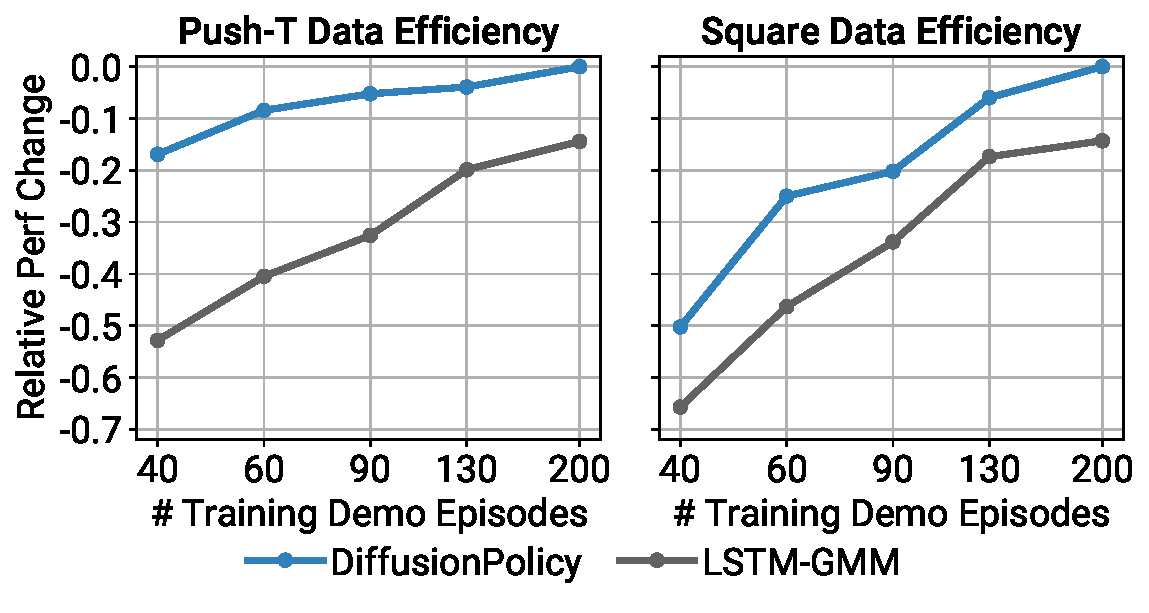
\includegraphics[width=\linewidth]{figure/sample_efficiency_figure.pdf}

\caption{\textbf{Data Efficiency.} 
\label{fig:data_efficiency}
Percentage change in success rate relative to the maximum (for both methods) is shown on the Y-axis.
% \textbf{Left}: trade-off between temporal consistency and responsiveness when selecting the action horizon. 
% \textbf{Right}: Diffusion Policy with position control is more robust against latency than velocity control.
% (b) The impact of observation horizon length on task performance.(d) Diffusion Policy is more sample efficient than BCRNN.
}
\end{figure}


\subsubsection{\textbf{Push-T}} 
\label{sec:eval_sim_pusht}
is a task we adopted from IBC \cite{ibc} to explore how Diffusion Policy work under the complex, contact-rich, and underactuated dynamics. The task is to push a T-shaped block (colored gray) into a fixed target pose (colored red) with a fixed circular end-effector (colored blue). The variation between episodes comes from the random initial condition for both the T block and the end-effector. Since the T block can only be pushed around by point contacts, the agent needs to exploit the object dynamics and constantly to change contact points and strategies to push the T block into a precise location. The task as two variants, one uses RGB image-based observation, and another is state-based, where 9 fixed 2D keypoints are computed from the ground truth pose for the T block. In addition, each variant also provides the current end-effector location for proprioception.

 \textbf{Evaluation Setup.}  The performance for each episode is measured by the maximum percentage of the green target region is covered by the T block. Following the original implementation, each episode auto-terminates when the coverage percentage reaches $95\% $, and the reported performance is normalized given $95 \%$ is the maximum possible coverage. Similar to RoboMimic tasks, the state-based experiments are trained for 4500 epochs and image-based experiments are trained for 3000 epochs. To report numbers in Tab \ref{tab:table_low_dim} and \ref{tab:table_image}, we also aggregated numbers across 3 training seeds and 50 environment seeds each.

\textbf{Result Analysis.} Diffusion policy  consistently outperforms other methods across all other methods, as shown in Tab \ref{tab:table_low_dim} and \ref{tab:table_image}. Similar to RoboMimic experiments, the difference between CNN and transformer-based Diffusion Policy on state-based tasks is small, but CNN is better on image-based tasks. We attribute this difference to the difficulty in tuning transformer models. This task also serves as a simulation testbed for our real-world Push-T task, where we use the same set of hyperparameters. \cheng{add link}. The demonstration data for this task is full of natural multimodality which is captured at different degrees by each method we tested, as shown in Fig \ref{fig:multimodal}. IBC \cite{ibc} also performs reasonably well and trails right after Diffusion Policy among the baseline methods, despite using exactly the same architecture and hyperparameters as what's used for RoboMimic experiments. We suspect IBC's performance difference between RoboMimic tasks and Push-T might be caused by their difference in action space dimension, where Push-T is only 2D while RoboMimic tasks are 7D or more.

\begin{table}[t]
\centering
% \includegraphics[width=0.45\linewidth]{example-image}~\includegraphics[width=0.45\linewidth]{example-image}
    % {Placeholder for thumbnails of each task}
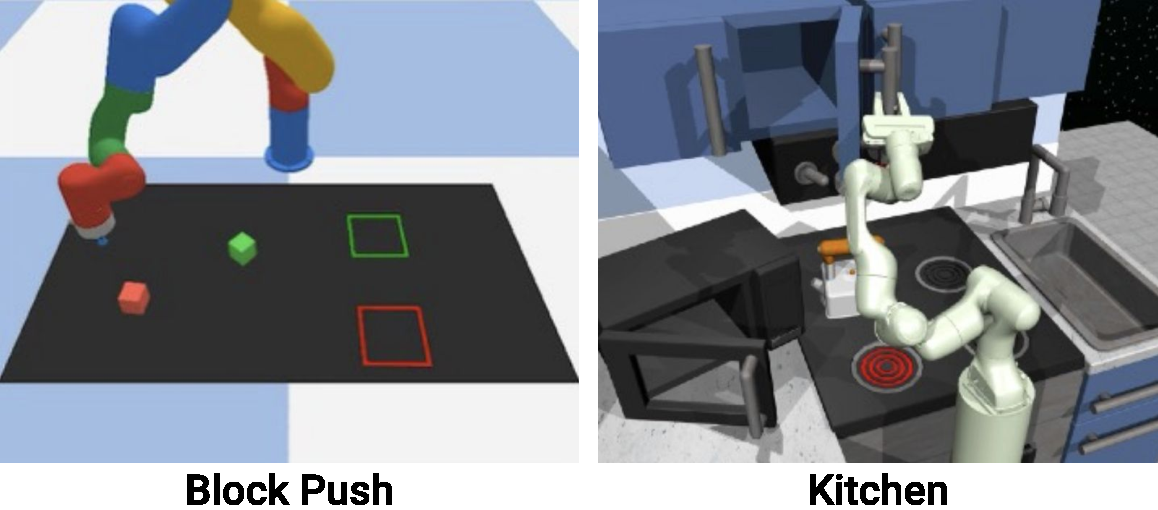
\includegraphics[width=0.9\linewidth]{figure/multitask_thumbnails.pdf}

\vspace{2mm}



\setlength\tabcolsep{4.8 pt}
\begin{tabular}{r|cc|cccc}
\toprule
 & \multicolumn{2}{c|}{BlockPush} & \multicolumn{4}{c}{Kitchen} \\
 & p1 & p2 & p1 & p2 & p3 & p4 \\
\midrule
LSTM-GMM & \small 0.03 & \small 0.01 & \small \textbf{1.00} & \small 0.90 & \small 0.74 & \small 0.34 \\
IBC & \small 0.01 & \small 0.00 & \small 0.99 & \small 0.87 & \small 0.61 & \small 0.24 \\
BET & \small 0.96 & \small 0.71 & \small 0.99 & \small 0.93 & \small 0.71 & \small 0.44 \\
DiffusionPolicy-C & \small 0.36 & \small 0.11 & \small \textbf{1.00} & \small \textbf{1.00} & \small \textbf{1.00} & \small \textbf{0.99} \\
DiffusionPolicy-T & \small \textbf{0.99} & \small \textbf{0.94} & \small \textbf{1.00} & \small 0.99 & \small 0.99 & \small 0.96 \\
\bottomrule
\end{tabular}

\caption{\textbf{Multi-Stage Tasks (State Observation)}. 
\label{tab:multi_stage}
For PushBlock, $px$ is the frequency of pushing $x$ blocks into the targets. 
For Kitchen, $px$ is the frequency of interacting with $x$ or more objects (e.g. bottom burner). 
Diffusion Policy performs better, especially for difficult metrics such as $p2$ for Block Pushing and $p4$ for Kitchen, as demonstrated by our results.
}
\end{table}

 
\subsection{Multi-Stage Benchmarks}
In this part of the experiment, we test Diffusion Policy on tasks that requires multiple distinct stages, while the order of the stage could be randomized, introducing long-horizon multimodal distributions in the demonstration data. 

\subsubsection{\textbf{Multimodal Block Pushing}} This task was adapted from BET \cite{bet}, which is specifically designed to test polices ability to model multimodal action distributions. The goal is to push two block into two squares in any order. The demostration data is generated by a scripted oracle policy that has access to groundtruth state information. The oracle policy has two stages: 1) randomly selects a block to push with $50\% $ possibility each and then pushes it to a randomly selected square with $50\% $ possibility each. 2) pushes the remaining block into the remaining square. This stochastic oracle creates multimodality in action sequence level (instead of the single-step level), which makes learning particularly challenging.

\textbf{Evaluation setup} Due to the two-stage nature of this task, we reported two metrics $p1$ and $p2$ which correspond to the frequency of pushing at least one or two blocks into the target squares. All methods are trained on 1000 demonstration episodes for 4500 epochs. The numbers for IBC and BET are copied from the original BET paper \cite{bet} since our reimplementation and experiments yield slighly worse performance. The numbers reported for Diffusion Policy and LSTM-GMM are averaged across 3 training seeds, 50 eval initial conditions for each and across 10 last checkpoints (1500 rollouts averaged in total).

\textbf{Result Analysis.} Transformer based Diffusion Policy beats BET \cite{bet} with significant margin on the $p2$ metric with 0.94 vs 0.71, as shown in Tab \ref{tab:multi_stage}. Other baselines performs very poorly on this task, where LSTM-GMM and IBC both has near 0 performance, demonstrating their inability to capture complex multimodal action distributions in practice. The CNN-based Diffusion Policy yields significantly lower performance compared to the transformer-based Diffusion Policy. This is likely due to CNN's inductive bias over-smoothing effects that removed the high-frequency signals presented in the oracle policy.

\subsubsection{\textbf{Kitchen}} has been widely used to demonstrate imitation learning or Offline RL algorithm's ability to learn long sequence action and multiple tasks simultaneously. The Relay Kitchen Environment \cite{gupta2019relay} contains in total of seven objects (hence tasks) to interact with: turning on the bottom or top burner, opening the hinge cabinet, moving the kettle, turning on the light switch, opening the microwave and sliding cabinet door. It also comes with a human demonstration dataset that contains 566 demonstrations, with the robot performing 4 tasks each in arbitrary order. The goal for evaluation is for the robot to execute as many of the demonstrated tasks as possible, regardless of their orders. This dataset not only contains both the \textbf{short-horizon multimodality} from humans on how to perform a task, but also the \textbf{long-horizon multimodality} on what tasks to perform. 

\textbf{Evaluation setup.} Similar to the Block Pushing task, we reported 5 metrics from $p1$ to $p5$, where each corresponds to the frequency for completing that number of tasks. Other training and reporting details are identical to that of the Block Pushing Task.

\textbf{Result Analysis.} Transformer-based Diffusion Policy again beats the best-performing baseline BET \cite{bet} by a significant margin on $p4$, demostrating its ability to capture both short and long horizon multimodality. The lower performance of the CNN-based Diffusion Policy is likely caused by the velocity control command action space for this task, which results in a high-frequency action signal, which is not favored by CNN's inductive bias.

\begin{table}[t]
\centering
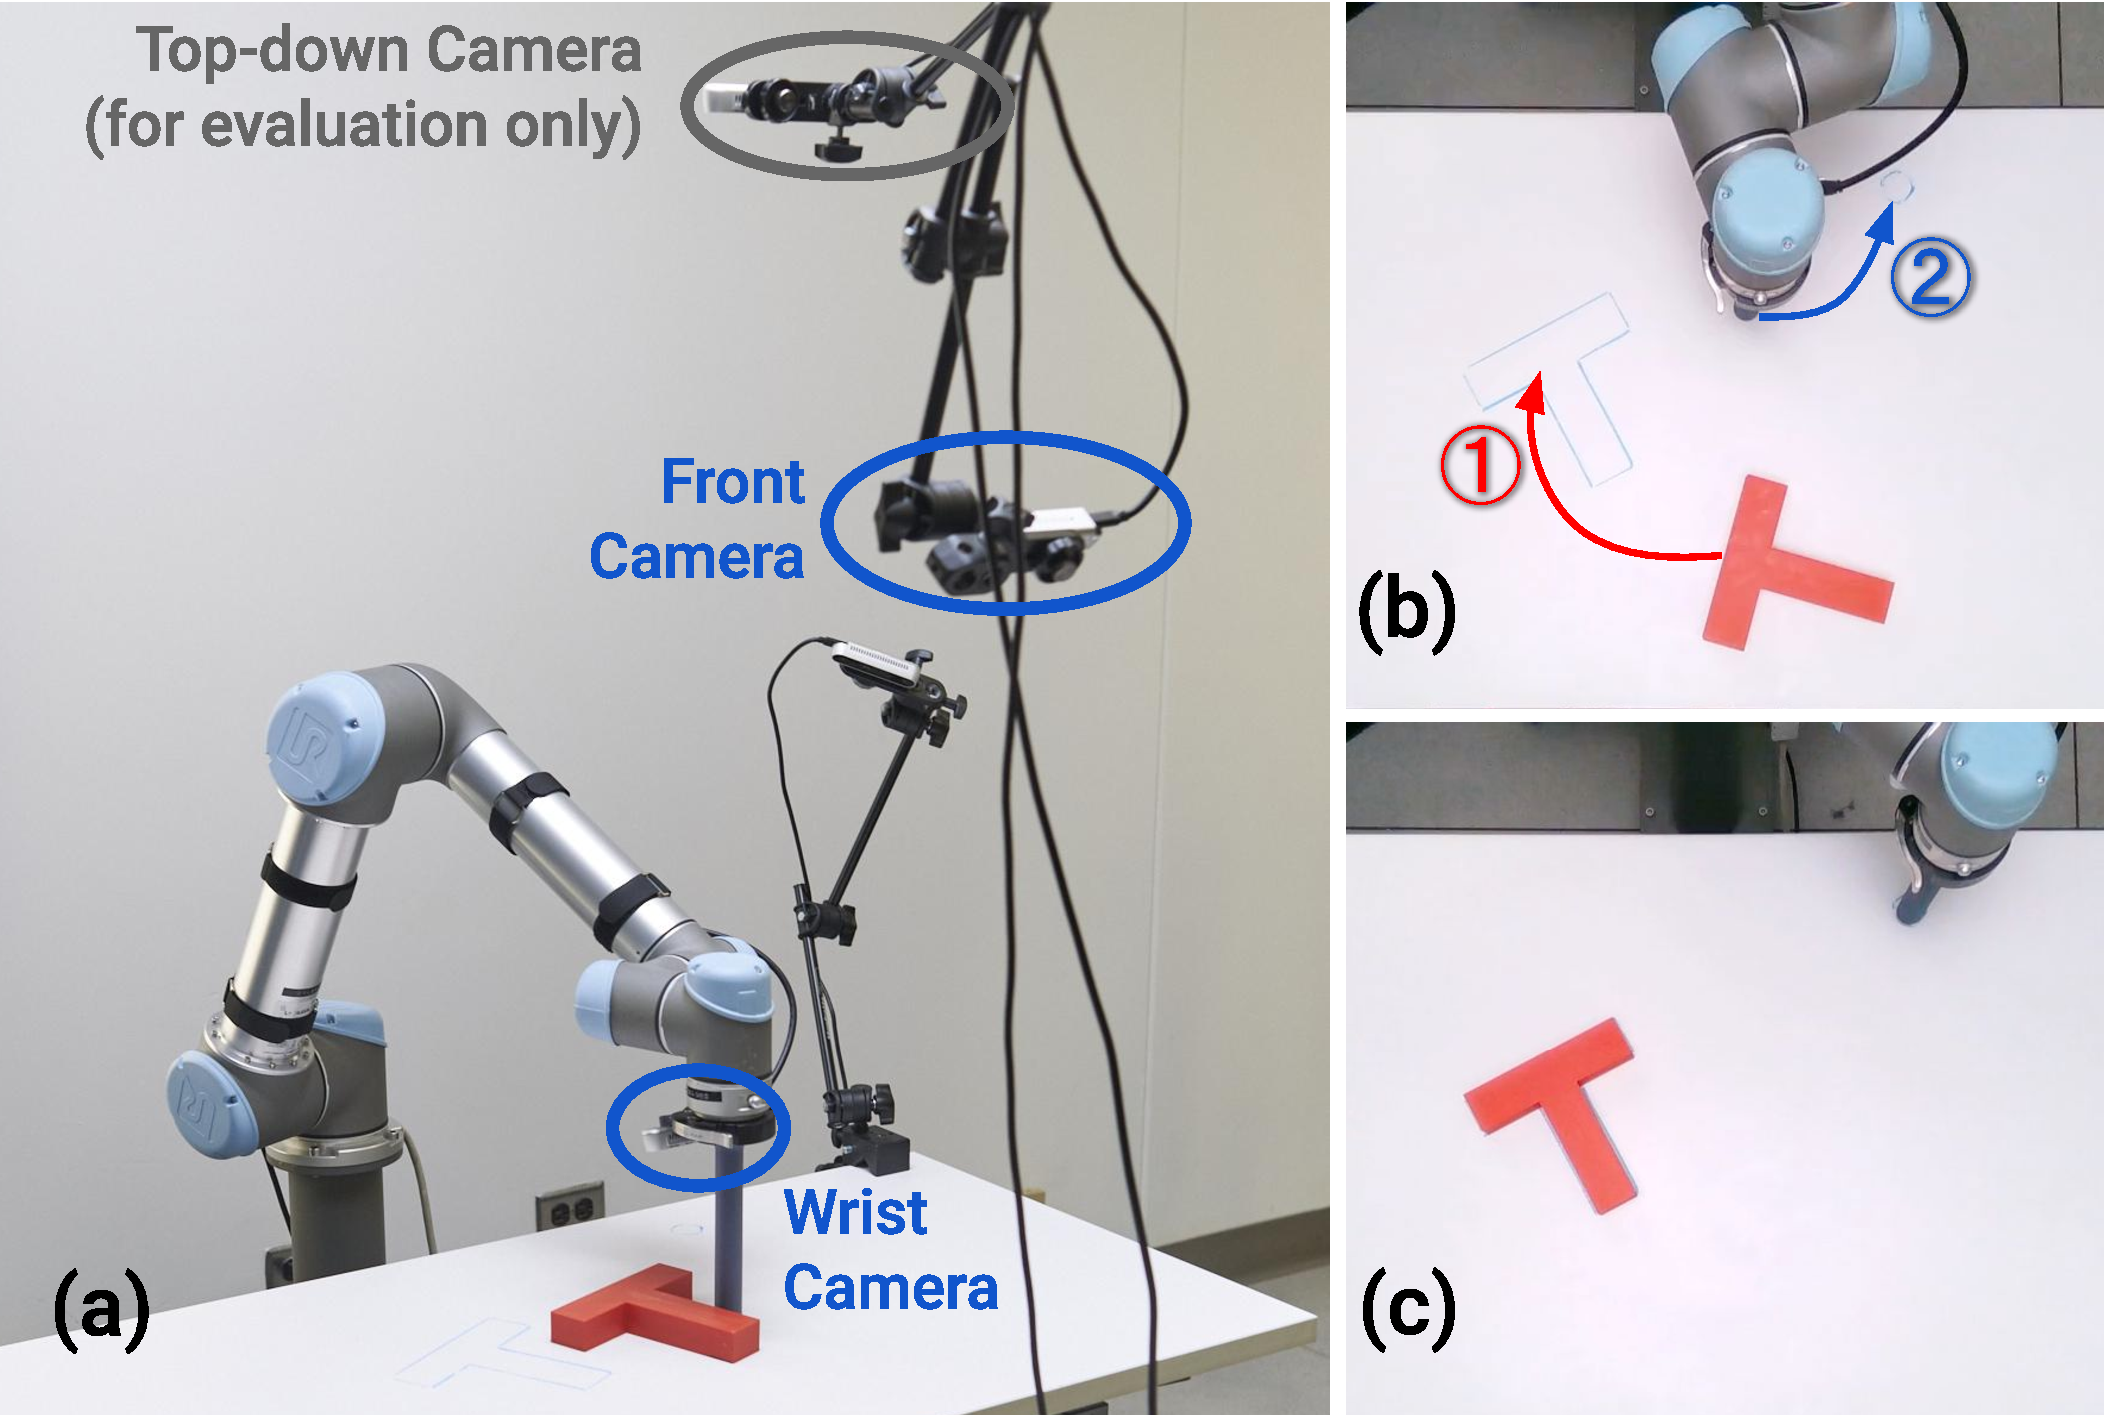
\includegraphics[width=0.9\linewidth]{figure/real_task_setup.pdf}
% https://docs.google.com/drawings/d/1LZCbfrzt3Ww82h2LQ9rt8BGS1fJCw5TyY-AnGr1RfjE/edit
% \label{fig:real_pusht_setup}

\vspace{2mm}
\setlength\tabcolsep{1.2pt}
\small
\begin{tabular}{c|c|cc|cc|cccc}
\toprule
       & Human & \multicolumn{2}{c|}{IBC} & \multicolumn{2}{c|}{LSTM-GMM} & \multicolumn{4}{c}{Diffusion Policy}     \\
       & Demo  & pos        & vel        & pos          & vel         & T-E2E & ImgNet & R3M & E2E         \\
\midrule
IoU      & 0.84  & 0.14       & 0.19       & 0.24         & 0.25        & 0.53  & 0.24     & 0.66  & \textbf{0.80} \\
Succ\%   & 1.00  & 0.00       & 0.00       & 0.20         & 0.10        & 0.65  & 0.15     & 0.80  & \textbf{0.95} \\
Dur. & 20.3  & 56.3       & 41.6       & 47.3         & 51.7        & 57.5  & 55.8     & 31.7  & \textbf{22.9} \\
\bottomrule
% https://docs.google.com/spreadsheets/d/1TftzQuEmERMvSM4EpzPl7GZ2mw5Ym024wV2TPW9N6R4/edit#gid=577907863
\end{tabular}


\caption{\textbf{Realworld Push-T Experiment.} 
\label{tab:real_pusht}
a) Hardware setup.  
b) Illustration of the task. The robot needs to \textcircled{\raisebox{-0.9pt}{1}} precisely push the T-shaped block into the target region, \textbf{and} \textcircled{\raisebox{-0.9pt}{2}} move the end-effector to the end-zone. 
c) The ground truth end state used to calculate IoU metrics used in this table. Table: Success is defined by the end-state IoU greater than the minimum IoU in the demonstration dataset. Average episode duration presented in seconds.}
\end{table}



\subsubsection{\textbf{Real-world Push T}}
\shuran{"Push-T" use consistent name, @Cheng. change it}
is the main real-world experiment that is used to study key design decisions in a real-world setup.  This task is inspired by the simulated Push T task, but with a few important modifications: 1) The real push-T \shuran{Push-T} task is \textbf{multi-stage}. The robot needs to first push the T block into the target, and then move the end-effector into a designated end-zone, as shown in Fig \ref{tab:real_pusht} (b) The end-zone is designed to avoid the robot's occlusion for the top-down evaluation camera. Avoiding occlusion is part of the task. 2) The policy has control over \textbf{episode termination}. By keeping the end-effector within the end-zone for more than 0.5 seconds, the evaluation episode is terminated. This requires the policy to decide when is the pose of the T block "good enough", which creates additional multimodality with its effect demonstrated in Fig \ref{fig:real_pusht_comparison}. Each episode also has a maximum time limit of 60 seconds. 3) The T block target IoU is measured at the \textbf{last step} for each episode, instead of taking maximum over all steps done in the simulated Push T task. Overall, these modifications makes the real-world Push T task more challenging that the simulated version.

\textbf{Hardware setup.} We used a UR5 robot with an cylindrical end-effector attachment to interact with the T block. The action sequences collected from demonstration and predicted by the polices have a frequency of 10Hz and is linearly interpolated to 125hz for robot execution. The action space is 2D in Cartesian space, with both positional and velocity control command experiment on some methods. The policy consumes 2 views of RGB image with 320 x 240 resolution for each at 10Hz. One camera is mounted in front of the experimental setup, and another is mounted on the 3D printed end-effector to get a closer look of the contact point between the robot end-effector and the T block, as shown in Fig \ref{tab:real_pusht}. An additional top-down camera is mounted specifically for computing IoU for the T block, and is not visible to the policies. The T block is also 3D printed with exterior dimension of 16cm x 16cm x 3cm.

\begin{figure*}
\centering
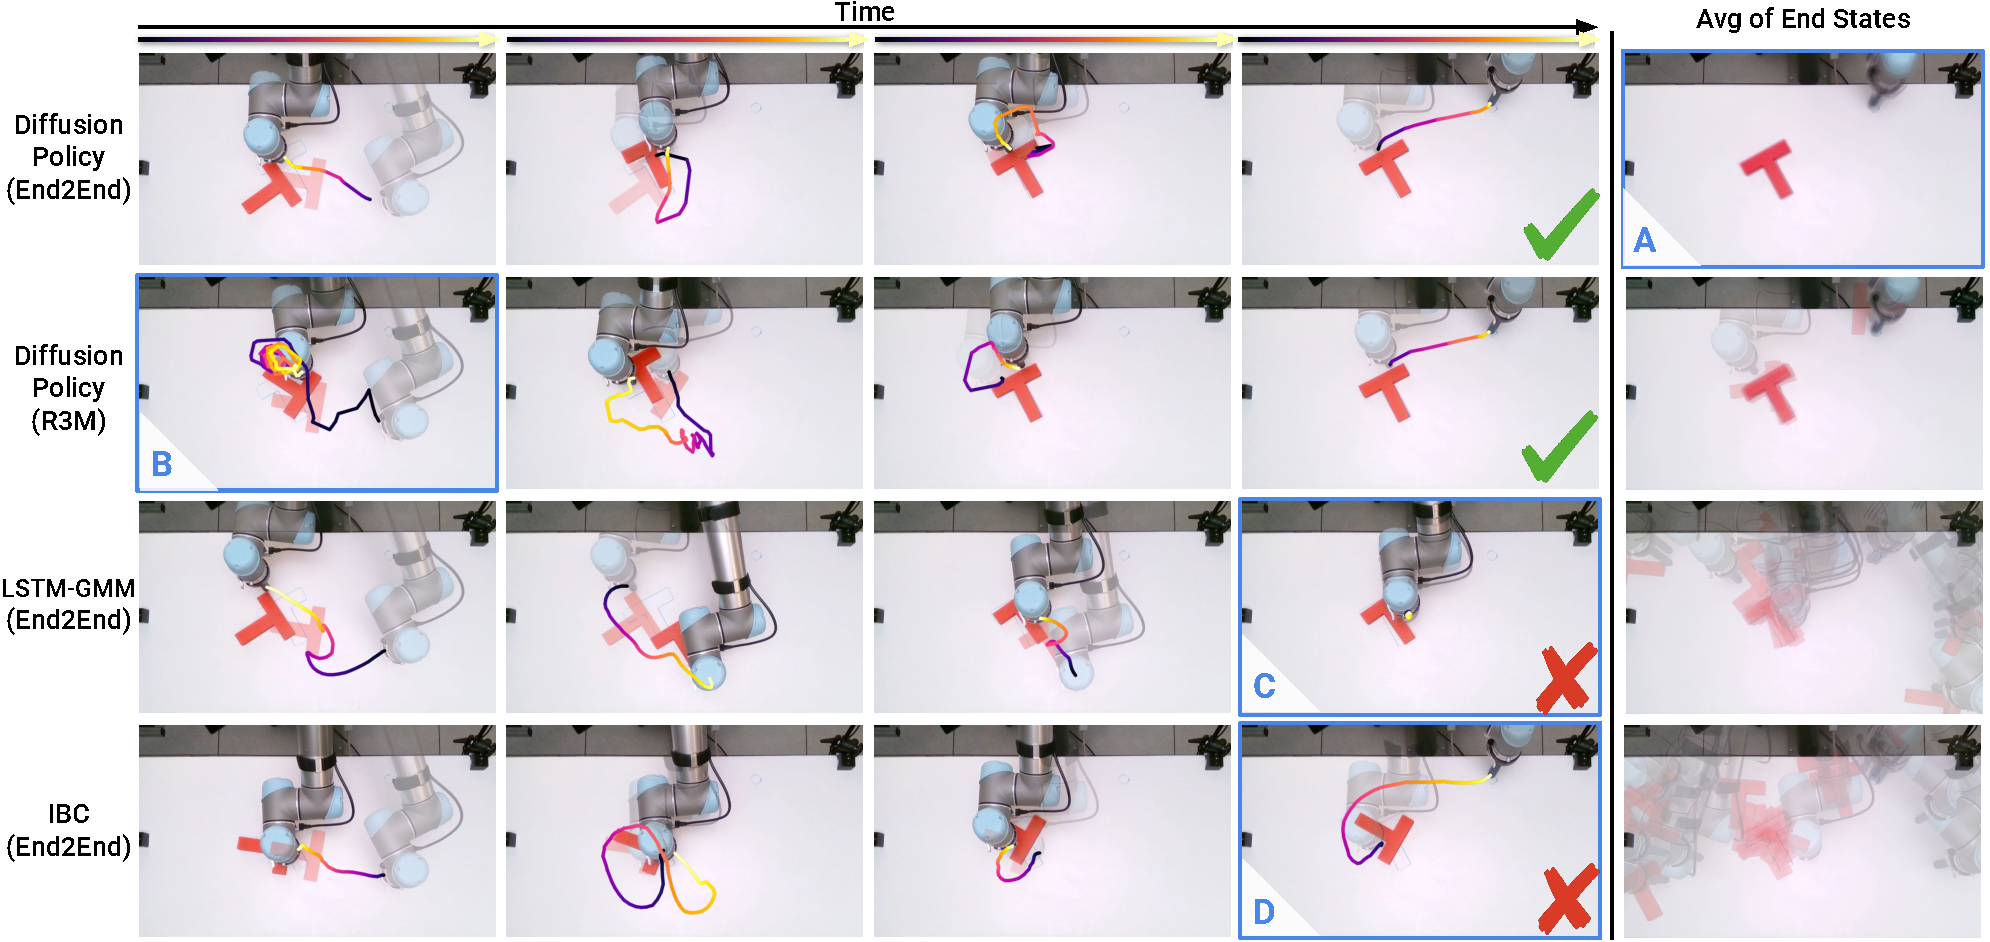
\includegraphics[width=\linewidth]{figure/real_results.pdf}

% https://docs.google.com/drawings/d/1LY-oKJ32jSTlIpMnEnoyYGfd58Il9Zzf-YhFS8Axin0/edit
\caption{\textbf{Realworld Push-T Comparisons.} 
\label{fig:real_pusht_comparison}
Columns 1-4 show action trajectory based on key events. The last column shows averaged images of the end state. 
\textbf{A}: Diffusion policy (End2End) achieves more accurate and consistent end states.
\textbf{B}: Diffusion Policy (R3M) gets stuck initially but later recovers and finishes the task. 
\textbf{C}: BCRNN fails to reach end zone while adjusting T block, blocking eval camera view.
\textbf{D}: IBC prematurely ends pushing stage.
}

\end{figure*}

\textbf{Evaluation setup.} 

 


All methods are trained on human collected demostration dataset with 136 episodes of pushing the T block from a random starting pose to its target. We used a fixed training time of 12 hours for each method, and selected the last checkpoint for each, with the exception of IBC, where the checkpoint with minimum training set action prediction MSE error due to IBC's training stability issue. The difficulty of training and checkpoint selection for IBC is demonstrated in Fig \ref{fig:ibc_stability}. Each method is evaluated for 20 episodes, all starting from the same set of initial conditions. To ensure the consistency of initial conditions, we carefully adjusted the pose of the T block and the robot according to overlayed images from the top-down camera. We reported 3 metrics, IoU (Intersection over Union), success rate and duration. The IoU is computed directly from the 1280x720 images from the top-down camera, with respect to a ground truth image of the desired pose for the T block, using binary masks computed using color filtering. The success rate is computed as the percentage of evaluation episodes where the IoU is higher than the lowest IoU in training demonstration dataset. 
% Since human demonstrations are also not perfect, the lowest IoU performance for demonstrations can act as an upper bound for the minimum acceptable performance. Since the policies also has control over episode termination, 
The episode duration is reported as a proxy for the self-termination performance of the evaluated methods.

\textbf{Result Analysis.} Looking across different methods, Diffusion Policy yields \textbf{close-to-human} performance with 95\%  success rate and 0.8 vs 0.84 average IoU, which is significantly higher than the best performing variants of IBC and LSTM-GMM baselines with 0\% and 20\% success rate respectively. Figure \ref{fig:real_pusht_comparison} qualitatively illustrate the behavior for each methods starting from the same initial condition. 
While Diffusion Policy straightforwardly reorient and adjusts the pose of the T block before heading to the end-zone (first row), both LSTM-GMM and IBC had difficulty on the transition between two stages of this task. In 8 out of 20 evaluation episodes, LSTM-GMM get stuck in near the T block while performing fine-adjustment for the T block's position, including the episode shown as the third row. On the other hand, IBC prematurely leaves the T block and head to the end-zone in 6 out of 20 evaluation episodes, including the episode shown as the fourth row. 
The behavior of LSTM-GMM and IBC suggests that the realworld Push T task is significantly harder due to its multi-stage nature and the \textbf{added multimodality} and uncertainty of deciding stage transition. 
Due to the slow and fine adjustments needed to achieve high accuracy for this task and the requirement to stay still in the end-zone to terminate episode, we did not follow the common practice to remove \textbf{idle actions} in the training dataset, which also contributes LSTM and IBC's tendency to get stuck in this task.
Consequently, the performance lead of Diffusion Policy under these challenges is greater that of the simulated push T task, shown in Tab \ref{tab:table_image}. 

\textbf{Effects of action space.} For LSTM-GMM and IBC baselines, we trained and tested both with positional and velocity control command action spaces. We found both method to predict highly jittery actions and yield lower IoU performance when used with positional control (shown in Tab \ref{tab:real_pusht}), which could explain why velocity control action space has been a popular choice for prior works in behavior cloning \cite{ibc,robomimic,bet}. However, we found Diffusion Policy (in particular the CNN based varaint) to perform better with positional control action space. In addition, positional control provides the advantage of being more robust against latency (shonw in Fig \ref{fig:ablation}) and allows greater precision when under low control frequencies. In realworld experiments, Diffusion Policy uses Action Horizon of $T_a=6$. Combined with the action frequency of 10Hz, the actual Diffusion Policy execution frequency is only 1.67 Hz. Despite the unusually low policy execution frequency, Diffusion Policy still yields consistently higher performance than baselines, enjoying the benefit the increased temporal action consistency and robustness against idle actions in the training dataset as discussed in Sec \ref{sec:action_sequence}.

\textbf{Effects of pre-trained vision encoders.}
We also experimented with pre-trained vision encoders for Diffusion Policy on this task by replacing the end-to-end trained ResNet-18 encoder with a frozen ImageNet \cite{deng2009imagenet} pretrained backbone or a frozen R3M encoder \cite{nair2022r3m} pretrained on Ego4D \cite{grauman2022ego4d}. Diffusion Policy trained with frozen pretrained vision backbones are slightly different in: 1) 224x224 images are accepted instead of the 320x240 resolution used for end-to-end, 2) the spatial softmax pooling end-to-end Diffusion Policy inherited from robomimic \cite{robomimic} is replaced by global average pooling from standard ResNet. We found Diffusion Policy with R3M to perform decently albiet lower than the end-to-end trained version. As shown in the second row of Fig \ref{fig:real_pusht_comparison}, we found Diffusion Policy-R3M to predict more jittery actions and get stuck more frequently than End-to-end trained version. However, Diffuison Policy-R3M often able to escape from getting stuck due to the stochastic nature of DDPM sampling. In contrast Diffusion Policy-ImageNet yield much less promising result, with even more jittery action prediction and sometimes moving abruptly to one corner of the table. From these experiments, we can conclude that training vision encoder \textbf{end-to-end} is still the most effective way to incorporate vision observation to Diffusion Policy, despite its data quantity disadvantage over pretrained models.

\begin{figure}[t]
\centering
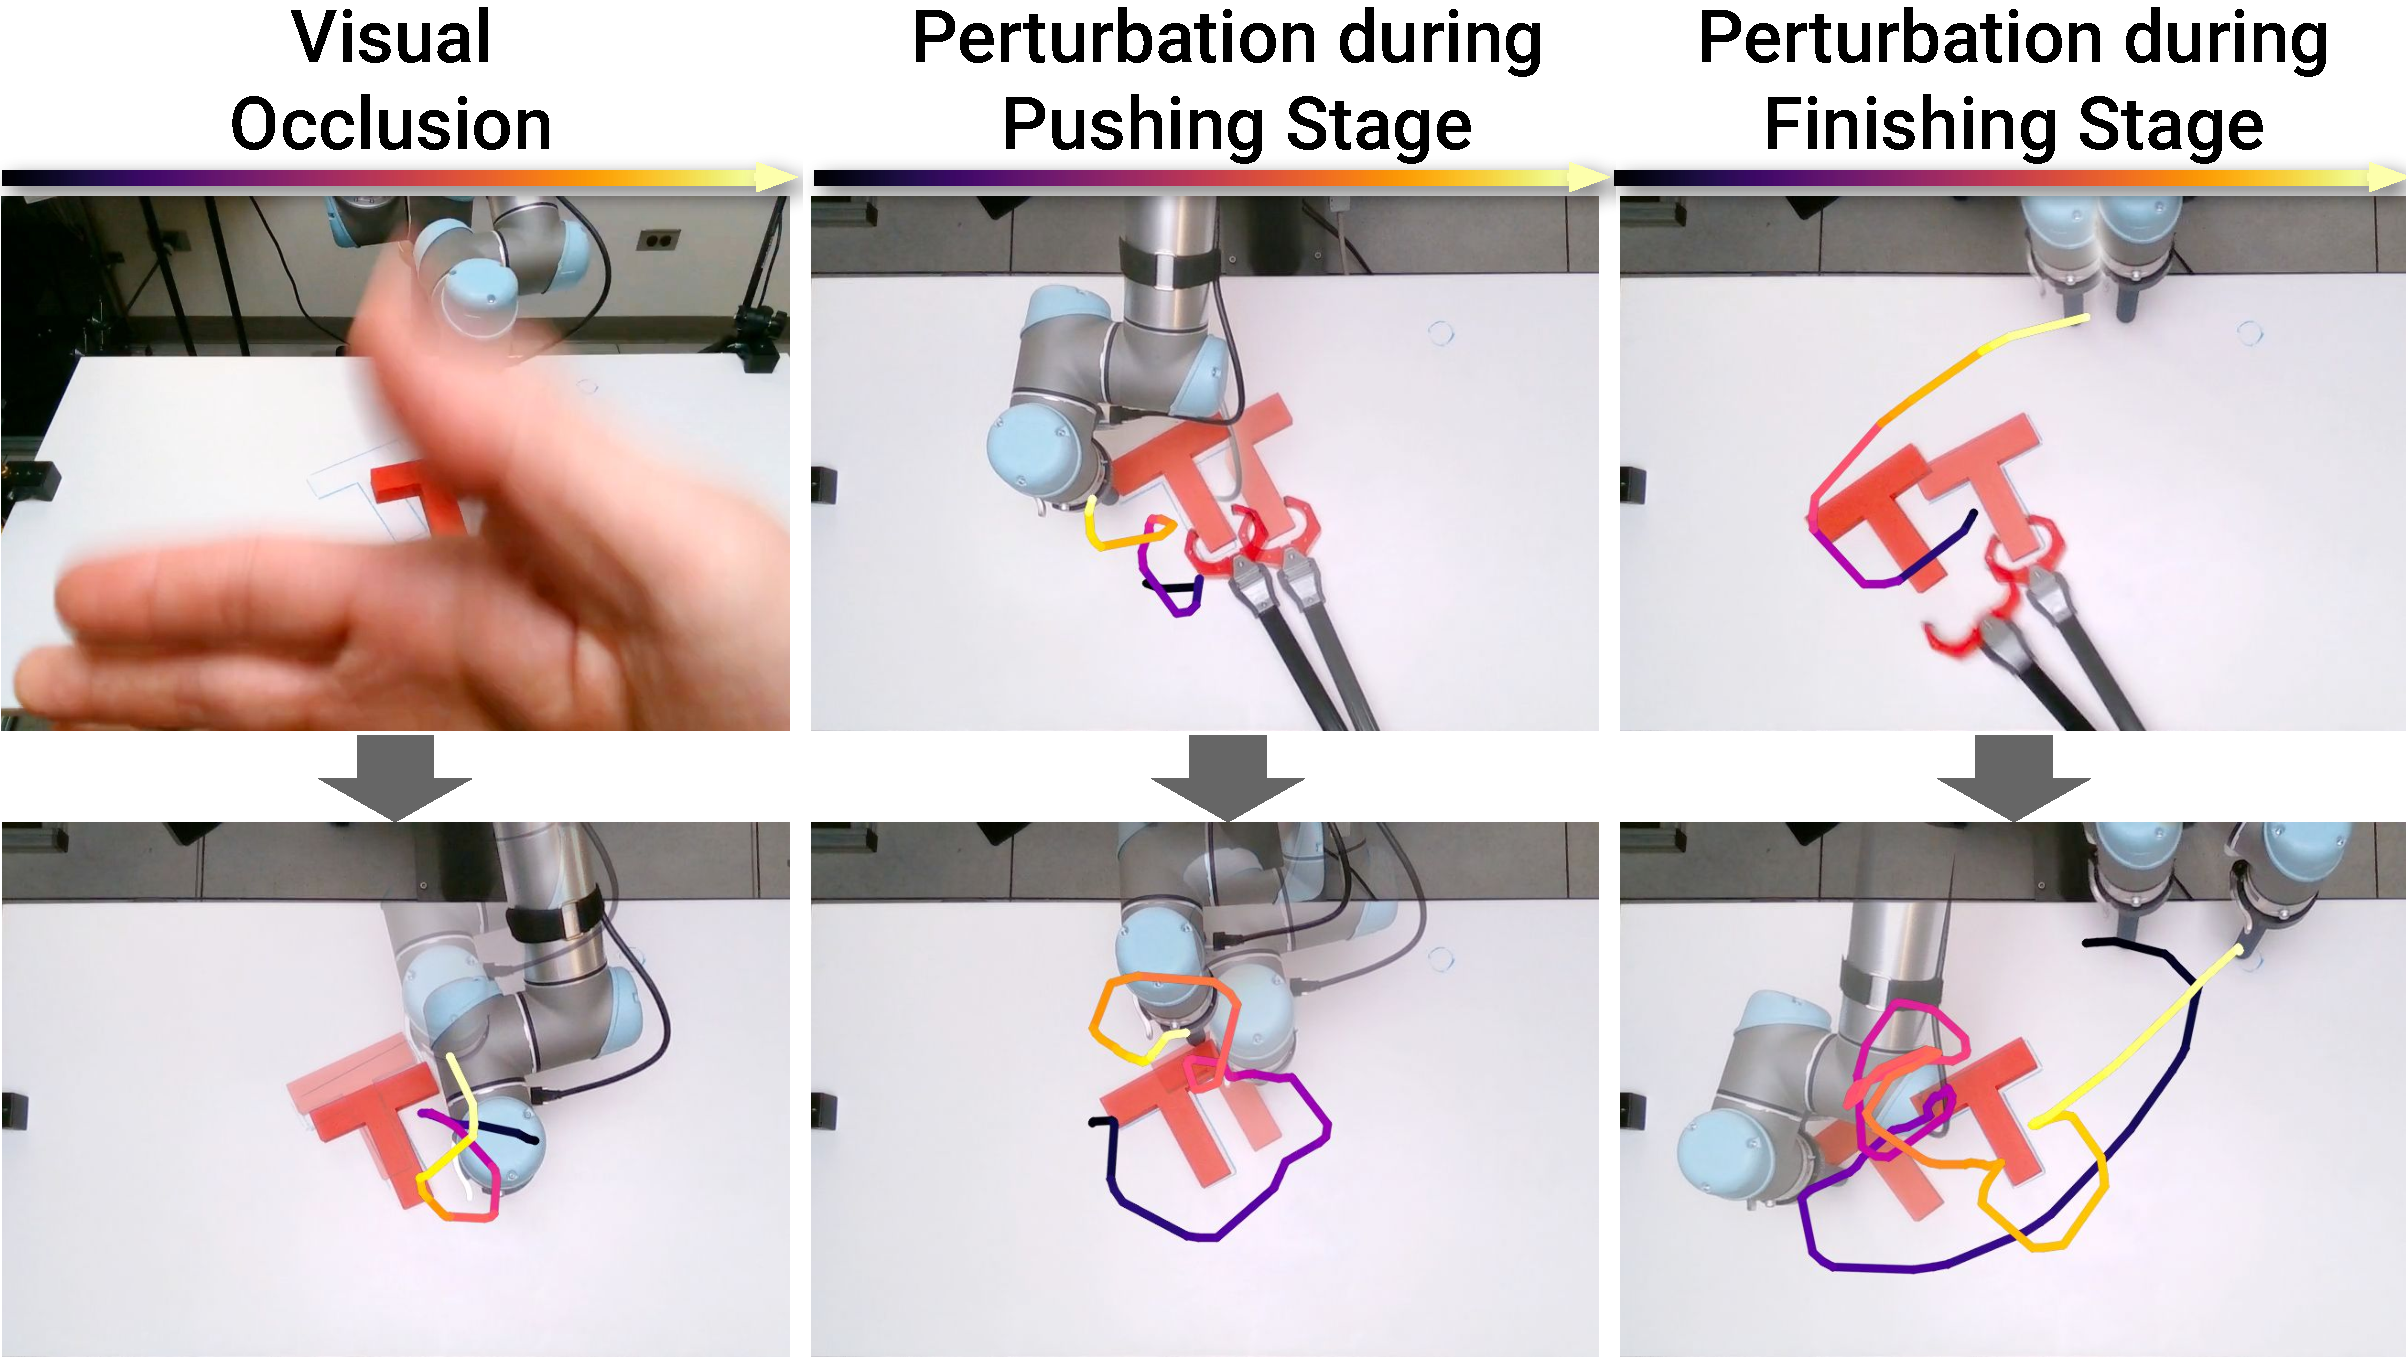
\includegraphics[width=\linewidth]{figure/real_robustness.pdf}

% https://docs.google.com/drawings/d/13XwTyXJvdaa6HUrVMTcfdnoLmYsXkhqscgtLth0J-zk/edit
\caption{\textbf{Robustness Test for Diffusion Policy.} 
\label{fig:robustness}
\textbf{Left}: Waving hand in front of camera for 3 seconds causes slight jitter, but the predicted actions still function as expected. 
% Left: Waving hand in front of the front camera for 3 seconds. The predicted actions are slightly jittery but still function as expected. 
\textbf{Middle}: Diffusion Policy immediately corrects shifted block position to goal state during pushing stage.
\textbf{Right}: Policy immediately aborts heading to end zone, returning block to goal state upon detecting block shift. This novel behavior was never demonstrated.
% Shifting the block while the policy has finished manipulating the block and is heading toward the end zone. The policy immediately aborts from moving to the end zone and moves the block back to the goal state. The behavior of aborting from heading to the end zone was never included in the demonstration. 
Videos in supplementary material.}
\vspace{-2mm}
\end{figure}

\subsection{Real-world Benchmarks}

\textbf{Robustness against perturbations.}
In a separate evaluation episode from the experiment to generate Tab \ref{tab:real_pusht}, we examine Diffusion Policy's robustness against visual and physical perturbations. As shown in Fig \ref{fig:robustness}, three types of perturbations are applied. Shown in the left column, the front camera is blocked by a quickly waving hand for 3 seconds. Diffusion policy predicts action with increased jitteryness, but was able to remain on-course to push the T block into position, which demonstrates the robustness of end-to-end trained vision encoders despite being trained without any augmentations. In the middle column, we shifted the T block while Diffusion Policy was fine-adjusting the T block's position. Diffusion policy immediately re-planed to push from the opposite direction, negating the impact of perturbation. In the right column, while the robot has pushed the T block in to the target and is en route to the end-zone, we moved the T block out of the target. Diffusion Policy immediately changed course back to adjust the T block back to its target, before proceeding to the end-zone. There is no demonstration in the training dataset that exhibits the behavior of going back to T block pushing while previously en route to the end zone. This experiment demonstrates that Diffusion Policy is able to \textbf{synthesize novel behavior} in the face of unseen observations.





\subsubsection{Real-world Sauce Manipulation Tasks}
\sfeng{write something about motivation for this task?}
This set of experiments were done on a robot station with two Franka Emika arms and two RealSence D415 cameras. Both tasks share the exact same setup during training and inference, with demonstration data being the only difference. The policy consumes both views (320 x 240) and end effector pose (6D rotation representation in \cite{zhou2019continuity}) as inputs, and commands end effector pose at 10hz. Similar to the PushT task, we used two separate ResNet18 encoders for each view, which are trained end-to-end with a CNN diffusion policy. For both tasks, 40 expert human demonstrations were used for training. Trained for 900 epochs.

\textbf{Pouring Evaluation}
Goal for this task is to pour one full ladle of sauce onto the center the pizza dough. Score is assigned by the IoU between the poured sauce mask and a nominal circle at the center of the pizza dough. Radius of the nominal circle is computed from the average poured sauce mask size from all the expert demonstrations. Since this task has more distinctive stages, we also assigned partial credits to roll outs that did not fully complete the task. 

\textbf{Spreading Evaluation}
Goal for this task is to evenly cover pizza dough with sauce. Amount of sauce is fixed during all training and evaluation runs. Score is assigned based on sauce coverage. 


\textbf{Result Analysis}




\begin{figure}[t]
\centering
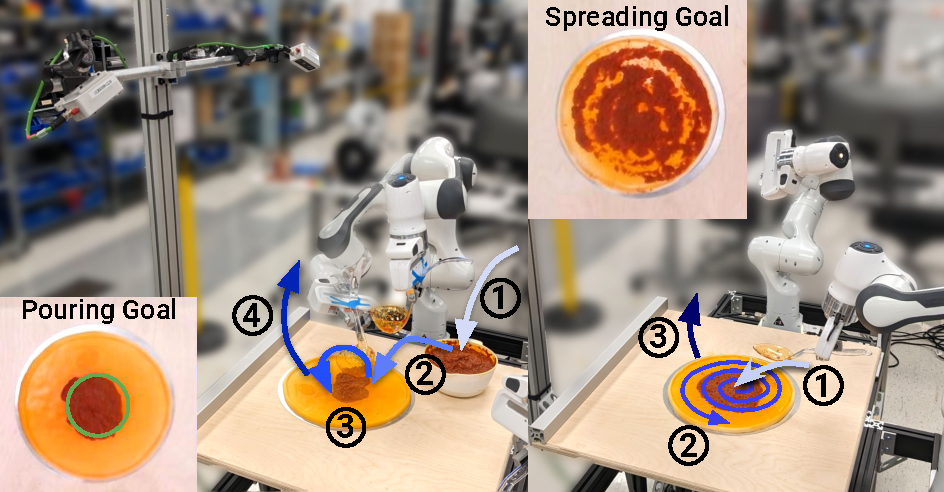
\includegraphics[width=\linewidth]{figure/real_sauce_setup.pdf}
% 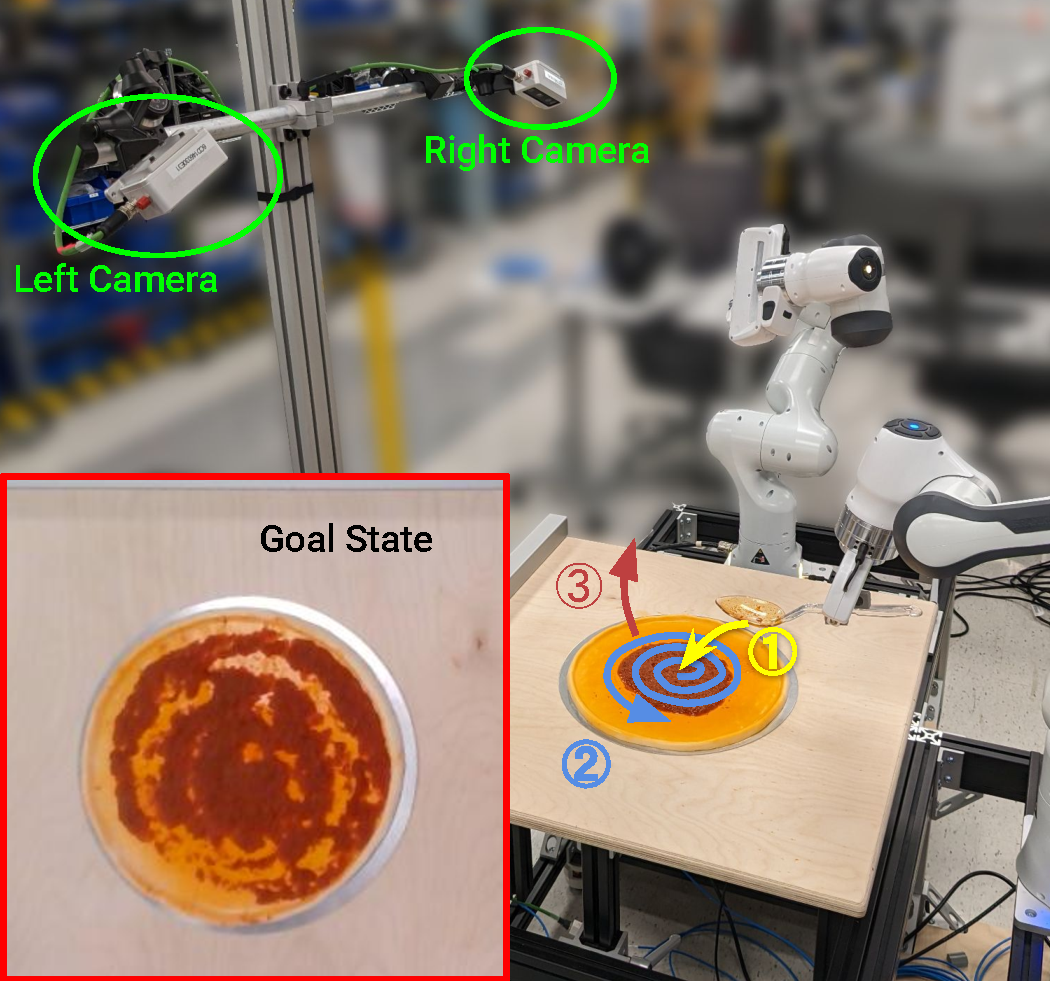
\includegraphics[width=0.5\linewidth]{figure/real_spreading.pdf}
% https://docs.google.com/drawings/d/1j7LKFAxZ2SXro3YbTC49KA1a7iuld-u5aY0oJHZzNUA/edit
% https://docs.google.com/drawings/d/1XDVS3JRA8forPWfl3t-7kVvTgDhtGlcqK0HsKyE-0Xc/edit

\vspace{2mm}


\small
\begin{tabular}{r|c|c|c|c}
\toprule
         & \multicolumn{2}{c|}{Pour} & \multicolumn{2}{c}{Spread}    \\
         & IoU & Succ & Coverage & Succ \% \\
\midrule
Human  & 0.79 &     1.00  & 0.79  &    1.00      \\
\midrule
LSTM-GMM & 0.06 & 0.00  &  0.27  & 0.00           \\
Diffusion Policy  &  \textbf{0.74} &\textbf{0.79}   & \textbf{0.77}  & \textbf{1.00}   \\
\bottomrule
\end{tabular}



\caption{\textbf{Realworld Sauce Manipulation. } 
% \todo{Update the table, double check the number} 
\todo{REPLACE picture during pouring}  
[Left] \textbf{Pouring Task.} The robot needs to \textcircled{\raisebox{-0.9pt}{1}} dip the ladle to scoop sauce from the bowl, \textcircled{\raisebox{-0.9pt}{2}} approach the center of the pizza dough, \textcircled{\raisebox{-0.9pt}{3}} pour sauce, and \textcircled{\raisebox{-0.9pt}{4}} lift the ladle to finish the task.
[Right] \textbf{Spreading Task} The robot needs to \textcircled{\raisebox{-0.9pt}{1}} approach the center of the sauce with a grasped spoon, \textcircled{\raisebox{-0.9pt}{2}} spread the sauce to cover pizza in a spiral pattern, and \textcircled{\raisebox{-0.9pt}{3}} lift the spoon to finish the task.
}
\end{figure}







